\documentclass{../../text-style}

\texttitle{Развёртывание, Docker}

\begin{document}

\maketitle
\thispagestyle{empty}

\section{Теоретическое введение}

В прошлый раз мы разработали на ASP.NET веб-приложение, но веб-приложения не особо полезны, если запускаются только на локальном компьютере. Поэтому рассмотрим технологии, которые позволят нам развернуть приложение, чтобы оно было доступно всем желающим: контейнеризацию и облачный хостинг.

Начнём с Docker, стандарта де-факто в контейнеризации\footnote{Docker --- не единственное решение для контейнеризации, стоит упомянуть также LXC (Linux Containers).}. Концептуально Docker --- это легковесная виртуальная машина, которая виртуализирует не машинные команды, как обычные виртуалки, а системные вызовы, то есть ядро операционной системы используется машины-хоста. Что хуже в плане изоляции, чем обычные виртуалки (например, вирусы в Docker-контейнерах запускать может быть плохой идеей), но гораздо быстрее. Ещё Docker-контейнеры отличаются от виртуалок тем, что в них работает один процесс (ну, это легко обойти, но концептуально контейнер --- это виртуализированный процесс, а не виртуализированная машина). И Docker-образы (то есть то, из чего запускаются контейнеры) только для чтения, то есть чтобы хранить в контейнере какие-то данные, надо отобразить его файловую систему на файловую систему хостовой машины. Тем не менее, Docker --- это стандарт де-факто по развёртыванию веб-приложений, потому что позволяет запустить готовое к работе приложение буквально одной командой. 

Почему --- в Docker-образе находится само виртуализированное приложение и все его зависимости, включая системные и прикладные библиотеки, нужные для работы файлы, настройки, переменные окружения и т.д., так что любой Docker-образ можно запустить одной командой, не заморачиваясь установкой и настройкой на целевой машине абсолютно ничего, кроме самого Docker. Более того, все зависимости всегда будут такими, какими они были при создании образа, даже если вышли новые версии библиотек и перестал поддерживаться компилятор --- пока образ доступен, его всегда можно будет запустить, и он будет в точности такой, как в момент создания.

Причём ещё есть Docker Hub, который что-то вроде GitHub для Docker-образов --- туда можно загрузить собранный Docker-образ, чтобы потом скачать на другой машине и запустить. Современные облачные провайдеры, чтобы задеплоить ваше приложение, могут попросить просто имя образа, сами укачают его с Docker Hub и запустят. Docker и Docker Hub, как и GitHub, бесплатны. Под Linux Docker поставить и настроить очень просто, под Windows, возможно, придётся повозиться --- если сделать это неправильно, он будет запускать VirtualBox, то есть настоящую виртуалку. Если сделать это правильно, придётся ставить WSL2 (к счастью, в Windows 11 она уже установлена) и терпеть исчезновение до 35 Гб места на диске. И ещё, возможно, включить HyperV в настройках BIOS (который давно уже называется UEFI, но традиции сильны), но это уж как повезёт, и как именно это сделать, зависит от производителя вашей материнской платы.

Docker-образ (Docker Image) --- это запускабельный образ приложения со всем окружением, необходимым ему для работы (можно понимать как очень навороченный .exe-файл). Образ состоит из слоёв, доступных только для чтения. Например, поверх слоя Alpine Linux лежит слой рантайма ASP.NET, поверх которого слой вашего веб-сервиса, поверх которого лежит слой конфигурации:

\begin{center}
    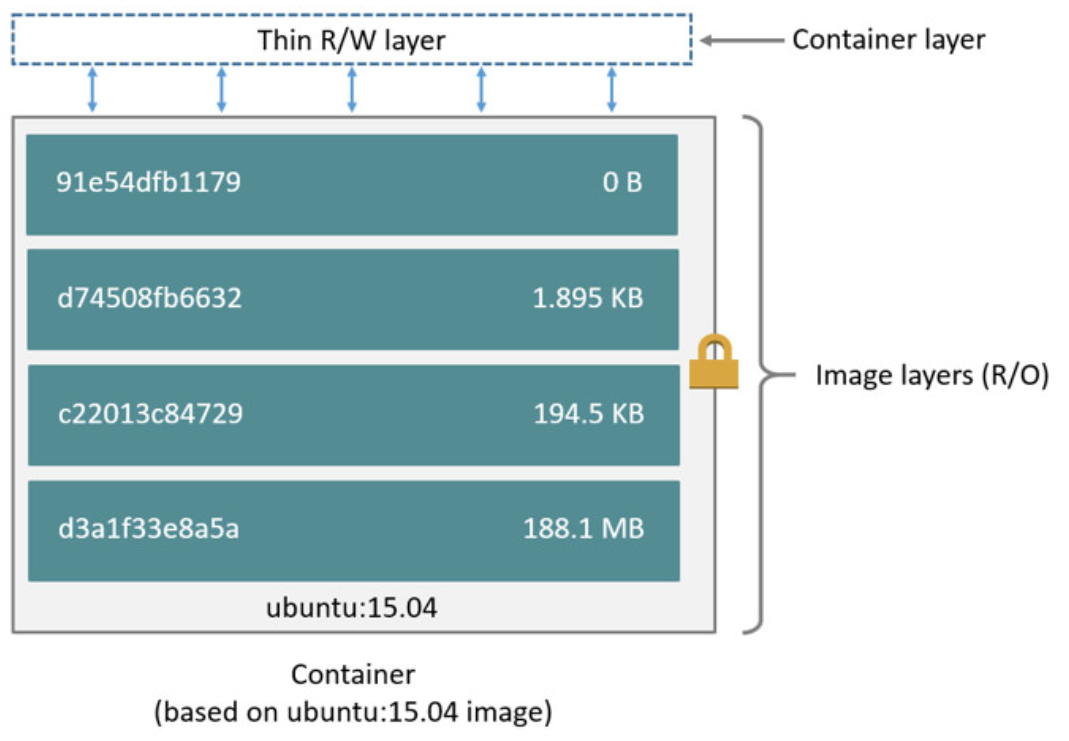
\includegraphics[width=0.5\textwidth]{dockerLayers.png}
    \attribution{\url{https://www.docker.com}}
\end{center}

Каждый слой имеет свою файловую систему и свои переменные окружения, и результирующая файловая система образа получается просто накладыванием слоёв последовательно один на другой (то есть если в слое A есть file1.txt и file2.txt, а в слое B file2.txt и file3.txt, в результирующем образе будет три файла). Поскольку слои read-only, образы могут разделять слои между собой, как процессы могут разделять динамические библиотеки. Так что, например, если у вас на машине 20 образов поверх Alpine Linux, то слой Alpine Linux у вас ровно один, что очень позитивно сказывается на объёме хранимых данных и потребляемом сетевом трафике (образы скачиваются послойно, так что если вы скачали слой один раз, он больше не качается).

Любой образ может служить базой для создания другого образа. Это, собственно, обычно и делается, когда вы собираете свой образ --- поверх всех слоёв существующего образа кладёте один или несколько своих слоёв.

Docker-контейнер (Docker Container) --- это запущенный экземпляр образа, типа запущенного .exe-файла:

\begin{center}
    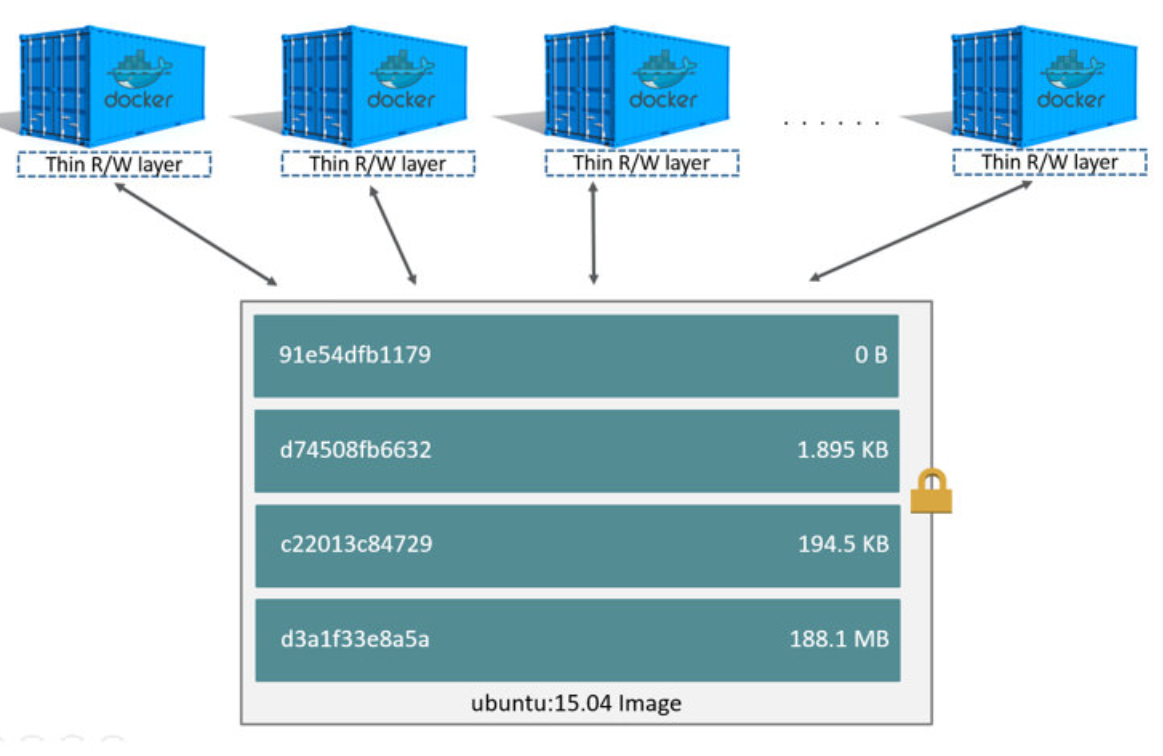
\includegraphics[width=0.6\textwidth]{dockerContainer.png}
    \attribution{\url{ https://www.docker.com}}
\end{center}

У контейнера есть дополнительный слой для записи, который может использоваться файловой системой внутри контейнера для хранения временных данных, но все изменения в нём гибнут при перезапуске контейнера (однако можно сохранить контейнер с его текущим состоянием файловой системы как новый образ). Контейнер содержит один запущенный процесс. Ничто не мешает этому процессу быть, например, bash, из которого запущено ещё десять процессов, но обычно в контейнере работает просто целевое приложение.

Терять данные при перезапуске контейнера, наверное, плохая идея, поэтому приложения, которым требуется хранение данных, должны использовать файловую систему хоста --- например, базы данных, запущенные в контейнере, должны хранить свои данные где-то ещё. Это можно сделать аж тремя способами:

\begin{center}
    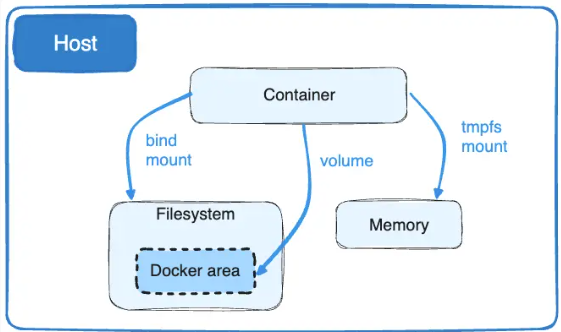
\includegraphics[width=0.6\textwidth]{persistence.png}
    \attribution{\url{ https://www.docker.com}}
\end{center}

Самый частоиспользуемый --- docker volume, файловое хранилище, которым управляет сам Docker. Его надо сначала создать командой \mintinline{text}|docker volume create <имя тома>|, которая в файловой системе хоста заведёт обычную папку. Командой \mintinline{text}|docker volume ls| можно просмотреть имеющиеся на локальной машине volume-ы, а \mintinline{text}|docker volume rm <имя тома>|. Подключить том к контейнеру можно при запуске, ключом \mintinline{text}|--mount|, например, \mintinline{text}|docker run -d --mount source=myvol,target=/app nginx:latest|.

\section{Процесс работы}

Собственно, предположим, что вы установили себе Docker. Что-то поделать с ним можно через Docker Desktop или вашу любимую среду разработки (скорее всего, она много чего умеет), но вообще docker --- это консольная утилита (даже две, docker daemon, запускающийся как сервис, и docker, консольный клиент для него). Вот самые основные команды:

\begin{itemize}
    \item docker run --- запускает контейнер. Если такого контейнера нет, делает pull, по умолчанию с Docker Hub. Основные аргументы:
    \begin{itemize}
        \item -d --- запустить в фоновом режиме. Без этого ключа docker не вернёт управление, пока контейнер не закончит работу, что может быть хорошо для отладки, но в боевом режиме не нужно;
        \item -p host\_port:container\_port --- прокинуть порт из контейнера на хост. Поскольку образы read-only, приложения в них сконфигурированы под некую абстрактную машину так, будто они на ней одни (например, слушают порт 80). Если запускаете два контейнера, каждый из которых слушает порт 80, случилась бы беда, поэтому docker сам симулирует сетевой стек и отображает порты хоста на порты контейнера в момент запуска контейнера. Так что какой порт выделить контейнеру, решает админ хоста, а не автор образа. По умолчанию все порты в контейнере закрыты, так что без ключа -p сетевое приложение запускать просто нет смысла.
        \item -i -t --- запустить в интерактивном режиме. Если в контенйере есть терминал, можно запустить его в интерактивном режиме, весь ввод с клавиатуры будет передаваться терминалу, а весь вывод --- вам в консоль, так что можно работать в контейнере так, будто вы подключились к удалённой машине по SSH. Очень удобно для отладки, но вручную что-то конфигурировать так в контейнере --- плохая идея, при перезапуске все изменения пропадут
        \item Пример: \mintinline{text}|docker run -it ubuntu /bin/bash|
    \end{itemize}
    \item docker ps --- показывает запущенные сейчас на хосте контейнеры с их id-шниками, по которым им можно потом посылать команды. Например, \mintinline{text}|docker run -d nginx; docker ps|
    \item docker stop --- останавливает контейнер (на самом деле шлёт SIGTERM, затем SIGKILL процессу в контейнере --- приложение внутри вправе проигнорировать эти сигналы);
    \item docker exec --- запускает дополнительный процесс в уже запущенном контейнере (если он там есть). В контейнеры очень редко ставят полноценный Linux с Bash, потому что они довольно большие, но есть набор утилит BusyBox, который словно бы создан для ручного ковыряния в контейнере --- размером он чуть более 2 мегабайт, но реализует все основные утилиты Unix, включая ash (Almquist Shell, легковесный, но не очень функциональный аналог bash). Поэтому если предполагается, что надо будет ходить внутрь контейнера, добавить туда слой с BusyBox может быть хорошей идеей.
\end{itemize}

\subsection{Dockerfile}

Чтобы собрать свой образ, потребуется Dockerfile --- это конфиг сборки контейнера, типа Makefile для Docker. Вот самый простой пример, из документации:

\begin{minted}{sh}
# Use an official Python runtime as a parent image
FROM python:2.7-slim

# Set the working directory to /app
WORKDIR /app

# Copy the current directory contents into the container at /app
ADD . /app

# Install any needed packages specified in requirements.txt
RUN pip install --trusted-host pypi.python.org -r requirements.txt

# Make port 80 available to the world outside this container
EXPOSE 80

# Define environment variable
ENV NAME World

# Run app.py when the container launches
CMD ["python", "app.py"]
\end{minted}

Команда FROM задаёт, на базе какого образа строится новый образ. Имя образа --- это собственно его имя, и \emph{тэг} после двоеточия. Тэг в принципе может быть любой строкой, но обычно используется \emph{semantic versioning} или специальные тэги типа latest.

WORKDIR --- это папка в файловой системе контейнера, которая будет рабочей для запускаемого процесса. 

ADD рекурсивно копирует содержимое указанной папки на хосте в файловую систему контейнера (тут мы копируем всю папку, где лежит Dockerfile, в папку /app в контейнере --- да, прямо в корень файловой системы, всё равно она больше никому, кроме нашего приложения, не будет видна).

RUN исполняет при сборке образа указанную команду \emph{внутри контейнера}. Тут мы менеджером пакетов Python ставим зависимости, которые заранее указали в requirements.txt.

EXPOSE открывает порт в контейнере (открываем порт 80).

ENV определяет переменную окружения, которая будет установлена в контейнере (самый простой способ управлять конфигурацией контейнера, благо переменные окружения можно переопределить при запуске).

Ну и последняя команда --- CMD, определяет, что надо запускать при старте контейнера. Тут запускается интерпретатор Python на указанный скрипт (из WORKDIR).

Вот несколько более интересный пример, типичного Dockerfile для типичного ASP.NET-приложения:

\begin{minted}{docker}
FROM mcr.microsoft.com/dotnet/aspnet:8.0 AS base
WORKDIR /app
EXPOSE 80
EXPOSE 443

FROM mcr.microsoft.com/dotnet/sdk:8.0 AS build
WORKDIR /src
COPY ["ConferenceRegistration.csproj", "."]
RUN dotnet restore "./ConferenceRegistration.csproj"
COPY . .
WORKDIR "/src/."
RUN dotnet build "ConferenceRegistration.csproj" -c Release -o /app/build

FROM build AS publish
RUN dotnet publish "ConferenceRegistration.csproj" -c Release -o /app/publish /p:UseAppHost=false

FROM base AS final
WORKDIR /app
COPY --from=publish /app/publish .
ENTRYPOINT ["dotnet", "ConferenceRegistration.dll"]
\end{minted}

Тут аж четыре команды FROM, что вызывает вопрос, на каком же образе основывается собираемый образ. Дело в том, что FROM сбрасывает текущее состояние образа, но AS позволяет запомнить это состояние как отдельный слой, который потом можно использовать. Итак, тут:

\begin{enumerate}
    \item Сначала берётся базовый образ с рантаймом ASP.NET, настраивается рабочая папка, открываются порты (HTTP и HTTPS, потому что веб-сервисов, не использующих HTTPS, практически не бывает).
    \item Затем в качестве базового выставляется образ с .NET SDK, куда копируется проектный файл и выполняется команда dotnet restore, скачивающая зависимости для проекта. 
    \item Затем поверх того, что получилось, копируются и остальные исходники, запускается сборка (командой dotnet build).
    \item Дальше создаём новый слой поверх результатов сборки, выполняем dotnet publish в нём, получая рабочее приложение со всеми зависимостями, сложенными в одну папку (наподобие make install).
    \item Дальше сбрасываем всё, возвращаясь к самому первому слою, и копируем из слоя publish собранное приложение в рабочую папку. В итоге получаем образ, в котором только рантайм ASP.NET (без всякого SDK) и собранное приложение с нужными ему библиотеками, никаких исходников или промежуточных файлов сборки.
    \item Дальше устанавливаем точку входа --- какой процесс будет запускаться (почти то же, что CMD, но CMD запускает шелл и передаёт ему указанные аргументы, а ENTRYPOINT сразу запускает процесс).
\end{enumerate}

Это называется <<двухфазная сборка>> (точнее, <<двухступенчатая>>), и это рекомендованная практика для сборки приложений на компилируемых языках. В принципе, нам ничего не мешает собрать приложение на хостовой машине и потом сложить в образ уже скомпилированные бинарники, но тогда на хосте надо будет иметь средства разработки, и если выйдет новая версия компилятора, которому не понравится наш код, то печаль. При сборке в самом образе инструментарий будет всегда именно таким, какой мы заказывали, он не будет зависеть от инструментов и окружения хостовой машины, вплоть до того, что такой образ можно собрать, имея только исходники и docker --- не надо не только иметь .NET SDK, но даже знать, что это такое. Работает как магия\footnote{На самом деле на этой магии основана практика контейнеризации рабочего места программиста, см. Docker Development Environments.}.

Dockerfile обычно кладётся рядом с .sln-файлом, в корне репозитория (ну или в папке с конкретной домашней работой). Чтобы собрать образ, надо запустить команду docker build с указанием папки, в которой лежит Dockerfile, и опционально названием результирующего образа. Например, \mintinline{text}|docker build -t conferenceregistration:latest .| --- собрать в текущей папке, где должен лежать Dockerfile, образ conferenceregistration с тэгом latest. Кстати, хоть latest по соглашению означает последнюю версию образа, включать в свой Dockerfile образы с тэгом latest считается очень плохой идеей, потому что при последующей сборке образа может прийти свежая версия внешней зависимости, с которой ваше приложение не тестировалось.

Кстати, в Visual Studio всё, что нужно, можно сгенерировать из среды разработки, либо указав при создании проекта необходимость создать Dockerfile, либо уже потом --- кликаем правой кнопкой по проекту, выбираем Add Docker Support, выбираем Target OS --- Linux (даже если у вас Windows, не пугайтесь, современная Windows умеет притворяться Linux-ом) --- потому что большинство реальных хостингов работают под Linux (точнее, чем-то UNIX-подобным), и хочется, чтобы на них контейнеры работали без проблем.

Дальше, если у вас есть Docker, можно запустить проект в Docker-контейнере через меню запуска (там, где можно выбрать хостиг и браузер). Оно соберёт образ (при этом написав в консоль, что оно делает, что приятно) и запустит контейнер из этого образа. По идее должно запуститься и работать как обычно.

А теперь давайте попробуем выложить получившийся образ на Docker Hub. Для этого там, естественно, надо завести аккаунт. Далее, кликаем правой кнопкой по проекту, выбираем Publish, выбираем Docker Container Registry, Docker Hub, вводим свои логин-пароль, жмём Publish. Оно снова соберёт образ и, по идее, зальёт его на Docker Hub. Если что-то пойдёт не так (или идея работать с Docker из среды разработки кажется вам унизительной), идём в консоль, набираем там docker images ls (отобразить список всех образов, что есть на машине), находим наш (например, conferenceregistration latest 2fdfa15fbf59 10 minutes ago 239MB). Сначала его надо переименовать в формат <имя пользователя>/<имя образа>, чтобы Docker Hub разрешил вам его пушить:

\begin{minted}{text}
docker image tag conferenceregistration:latest 
    <ваш юзернейм на Docker Hub>/conferenceregistration:latest
\end{minted}

(в одну строчку). Дальше, собственно, пушим на Docker Hub (перед этим по идее надо авторизоваться через Docker Desktop, но могут и при пуше попросить логин/пароль, я не помню):

\begin{minted}{text}
docker push <ваш юзернейм на Docker Hub>/conferenceregistration:latest
\end{minted}

И всё, через некоторое время образ зальётся, можно зайти на Docker Hub и проверить, что образ появился. Теперь вы можете пойти на другую машину, где есть Docker (например, одногруппника) и скачать/запустить ваш образ:

\begin{minted}{text}
docker run -d -p 80:80 <ваш юзернейм на Docker Hub>/conferenceregistration:latest
\end{minted}

Теперь можно просто в адресной строке браузера набрать localhost, и попасть в наше приложение (либо в Docker Desktop найти запущенный контейнер, посмотреть его логи и нажать на <<открыть в браузере>>). Собственно ключ -p у команды docker run прокидывает порт 80 контейнера на 80 порт вашей машины (а ключ -d (detach) говорит, что надо вернуть управление в консоль после старта контейнера). Прокидывание портов делается при запуске, чтобы если у вас на машине надо запустить 20 контейнеров, каждый из которых работает на порту 80, вы могли бы их раскидать сами по портам, не пересобирая контейнер.

\section{Развёртывание в облаке}

И наконец, выложим наше барахло на облачный хостинг, в нашем случае на Yandex Cloud (вообще, Amazon был бы выбором по умолчанию, либо Azure, раз уж .NET, но все они не очень любят теперь пользователей из России).

Yandex Cloud --- довольно типичный облачный хостинг, который умеет многие обычные для облачных хостингов вещи:

\begin{itemize}
    \item виртуальные машины в облаке --- когда вы арендуете виртуальную машину с предустановленной операционной системой и требуемыми аппаратными ресурсами (от которых сильно зависит стоимость) и сами ставите на неё всё, что нужно, и запускаете там что угодно; так долгое время в основном облачные хостинги и использовались;
    \item Cloud Functions --- диаметрально противоположный подход, вы заливаете код с функцией (например, на Python), хостинг сам превращает её в некое подобие веб-сервиса и берёт с вас деньги за её вызовы;
    \item облачные СУБД --- тут вы арендуете фактически connection string к уже настроенной базе данных и место для хранения; поддерживается много разных СУБД, и у Яндекса даже есть своя СУБД ClickHouse, которую они активно продвигают;
    \item сервис для распознавание/синтеза речи;
    \item разные ML-инструменты, тоже уже в виде преднастроенных сервисов --- кстати, можно арендовать хорошие видеокарты для работы с нейросетями;
    \item CDN и другие сетевые сервисы.
\end{itemize}

Нам в контексте деплоя интереснее всего сервис Serverless Containers --- аренда возможности запуска Docker-образов в облаке без всяких виртуалок. Плюс Yandex Container Registry --- хранилище для этих самых образов. Serverless Containers вроде как не умеют забирать образы с DockerHub (и, скорее всего, не хотят, чтобы не платить за трафик) и ожидают, что все используемые образы будут лежать в YCR.

Хорошая новость в том, что Yandex Cloud многие услуги для небольших проектов предоставляет бесплатно (например, до миллиона вызовов Cloud Functions), кроме того, предлагает стартовый грант, где новым аккаунтам даётся энное количество денег попробовать даже платные функции (правда, вроде бы на ограниченное время, около трёх месяцев). Для наших целей достаточно бесплатного уровня почти всего --- только YCR берёт деньги за хранение образов, сколь бы маленькими они ни были. Но деньги чисто символические, если вы не крупная компания с миллионом образов по гигабайту каждый --- автор сего текста укладывался в 5 копеек в месяц (!) для всех своих нужд. Деньги можно платить из стартового гранта, но может потребоваться привязать банковскую карту (как вообще принято у облачных сервисов) --- и поскольку при отсутствии опыта в подобных вещах может быть сложно предугадать месячные траты, имеет смысл иметь отдельную карту для оплаты услуг облачного сервиса.

\subsection{Развёртывание ConferenceRegistration}

Попробуем развернуть наше демо-приложение в Yandex Serverless Containers. Для этого сначала надо создать аккаунт на Yandex Cloud через \url{https://console.cloud.yandex.ru}. Там ещё попросят завести свою организацию, создаём какую попало --- каждый пользователь принадлежит организации, это особенность платформы. Затем надо создать новое облако и каталог (облако --- это абстракция облачных ресурсов аккаунта, каталог --- группа ресурсов; облака изолированы друг от друга, каталоги принадлежат облакам). Затем надо создать реестр Docker-образов и выложить туда образ нашего приложения, для этого:

\begin{itemize}
    \item ставим себе локально Yandex Cloud CLI --- консольный инструмент для удалённого управления облачными ресурсами, у всех облачных провайдеров что-то такое есть и нужно прежде всего для автоматизации всяких DevOps-задач; реестр можно создать и через веб-интерфейс, но Yandex Cloud CLI нам ещё пригодится;
    \item делаем yc init, авторизуемся в Yandex Cloud;
    \item создаём реестр Docker-образов: \mintinline{text}|yc container registry create --name <произвольное имя реестра>|;
    \item конфигурируем Docker для работы с YCR: \mintinline{text}|yc container registry configure-docker| --- теперь Docker будет уметь пушить образы в YCR, а не только на DockerHub, и правильно авторизоваться;
    \item присваиваем нашему образу тэг специального вида: \mintinline{text}|cr.yandex/<ID реестра>/<имя Docker-образа>:<тег>| --- это нужно, чтобы Docker знал, куда слать образ; ID реестра можно найти в веб-интерфейсе \url{https://console.cloud.yandex.ru};
    \item пушим образ в YCR обычной командой docker push, указывая как имя образа тэг из предыдущего пункта, например: \mintinline{text}|docker push cr.yandex/crpc9qeoft236r8tfalm/ubuntu:hello|;
    \item идём в \url{https://console.cloud.yandex.ru} и проверяем, что образ появился в реестре --- обратите внимание, что следующий push этого же образа создаст ещё одну версию, и все версии хранятся в реестре.
\end{itemize}

Теперь у нас есть образ в реестре, и надо сделать из него запускаемое приложение. Для этого снова идём в \url{https://console.cloud.yandex.ru}, выбираем там в меню каталога Serverless Containers, жмём <<Создать>>, вводим имя и описание приложения. Появляется страница, на которой можно указать требуемые ресурсы --- для наших целей можно выставить всё по минимуму, и это, скорее всего,позволит исполнять приложение совершенно бесплатно, хоть и небыстро. Самая важная настройка тут --- <<URL образа>>, тут мы выбираем образ из YCR, который будет запускаться в контейнере. Плюс нам потребуется <<Сервисный аккаунт>> --- аккаунт, от имени которого будет выполняться pull образа из YCR и запуск приложения при обращении пользователей по URL. Тут нам надо создать новый, но вообще одного для нескольких приложений достаточно. Дальше жмём на <<Создать ревизию>>, и через некоторое время новое приложение появится в списке контейнеров. Если на него кликнуть, покажутся детали приложения, включая URL, по которому в него можно попасть. Кликаем по нему --- и, если всё пойдёт хорошо, увидим наше приложение. И вот по этому URL туда может ходить по идее кто угодно (ну, если хотите красивый URL, можно использовать сокращалки ссылок типа bit.ly или заморочиться и арендовать себе доменное имя).

Пара опасностей, подстерегающих неопытных пользователей --- при выкладывании новой версии образа в YCR надо пойти в приложение и сказать ему, чтобы оно использовало эту новую версию (что логично, мы не хотим, чтобы в production что-то попадало само собой). И ещё отдаваемая пользователю приложением страница не должна быть больше 3Мб, это техническое ограничение Yandex Cloud, которое даже платным аккаунтом не преодолеть --- это может быть проблемой при активном использовании WebAssembly, например, в Blazor.

\section{Docker Compose}

Если у нас один контейнер, всё понятно. Но большинство практически полезных приложений состоят из нескольких контейнеров --- в самом простом случае само приложение и база данных, часто появляются другие зависимости (nginx, например), часто и само приложение разделяют на части (микросервисы). Можно было бы руками запускать все контейнеры через docker run, следить, что никто из них не упал, и настраивать каждому конфигурацию (например, видимо, порты надо будет как-то передавать всем запущенным контейнерам), и это может очень быстро надоесть. На помощь приходят \emph{оркестраторы}, один из которых, Docker Compose, поставляется прямо вместе с Docker. Вот пример конфигурации многоконтейнерного приложения, описываемого в файле compose.yaml\footnote{Взято с \url{https://github.com/docker/multi-container-app} (дата обращения: 03.12.2023).}: 

\begin{minted}{yaml}
services:
  todo-app:
    build:
      context: ./app
    depends_on:
      - todo-database
    environment:
      NODE_ENV: production
    ports:
      - 3000:3000
      - 35729:35729
  todo-database:
    image: mongo:6
    volumes: 
      - database:/data/db
    ports:
      - 27017:27017
\end{minted}

Тут говорится, что у нас есть два контейнера, один из которых собирается при старте из папки app, второй --- готовый образ mongo версии 6, причём первый зависит от второго (то есть будет пытаться запуститься только когда второй запустится). Контейнеру todo-app выставляется переменная окружения NODE\_ENV (это в дополнение к тем, что выставляются в его Dockerfile --- кстати, в папке app должен быть Dockerfile, иначе ничего не выйдет, Docker Compose оркестрирует готовые образы, сам их не собирает), в ports --- прокидывание портов, как в ключе -p для docker run. todo-database ещё определяет том для хранения данных (что логично, СУБД в памяти не очень надёжна).

Вот несколько более сложный, но более реальный пример, из одного из кафедральных студпроектов:

\begin{minted}{yaml}
services:
  web:
    container_name: web
    image: example/web-part:latest
    ports:
      - "5000:5000"
    depends_on:
      - gateway
    deploy:
      resources:
        limits:
          memory: 50M
        reservations:
          memory: 20M
    networks:
      - network-services
  gateway:
    container_name: gateway
    image: docker.pkg.github.com/example-gateway:master
    ports:
      - "8000:80"
    depends_on:
      - repo
      - auth
    networks:
      - network-services
  auth:
    container_name: auth
    image: docker.pkg.github.com/example-auth:master
    ports:
      - "8002:80"
    volumes:
      - type: bind
        source: ./Auth/users.db
        target: /users.db
    networks:
      - network-services
  repo:
    container_name: repo
    image: docker.pkg.github.com/example-repo:master
    ports:
      - "8004:80"
    networks:
      - network-services
networks:
  network-services:
    driver: bridge
\end{minted}

В любом случае, чтобы это всё запустить, надо использовать команду \mintinline{text}|docker compose up| в папке, где лежит compose.yaml (или docker-compose.yml). \mintinline{text}|docker compose up -d| запустит контейнеры в асинхронном режиме, то есть вернёт управление в консоль сразу. Остановить запущенные контейнеры можно командой \mintinline{text}|docker compose down| или через Docker Desktop.

Docker Compose на самом деле много чего умеет, даже собирать машины в кластер и балансировать нагрузку (поищите информацию про Docker Swarm, если интересно), однако для более взрослых задач обычно используют Kubernetes --- гораздо более сложный в настройке, но и гораздо более продвинутый оркестратор (который, кстати, тоже поставляется с Docker Desktop, так что у вас, скорее всего, уже установлен). Yandex Serverless Containers умеет Kubernetes, но не умеет пока Docker Compose, и вообще Docker Compose обычно слабо поддержан облачными провайдерами, потому что если вы хотите деплоить приложения в облаке, то вы хотите и Kubernetes. Однако кластер Kubernetes даже из одного узла стоит бешеных денег, поэтому первое время стоит, наверное, обходиться одним контейнером или деплоиться через Docker  Compose на облачную виртуалку. Тут Yandex Cloud предлагает Container Optimized Image --- виртуалку с настроенным Docker и Docker Compose, однако, как и все виртуалки, оно стоит уже несимволических денег (впрочем, всё равно в разы дешевле Kubernetes-кластера в облаке).

\end{document}
